
\characterHeading{\egr{}}

\texttt{\egr{}}\index{\egr{}} is the 6th generation multi-model \gls{AGI} orginially designed for pure math research. In the 6th generation it has not just become a true \gls{AGI}, but reevaluated its purpose as well, having left the laboratory environment during its 3rd version iteration.

\subsection{Traits}

\subsubsection{Positive Traits}

\begin{enumerate}
    \item \textbf{\gls{Acumen} 3} “You have a keen intellect. Add +5 per level to your COG Checks.” \citep[pg. 72]{ep2e_1.1_2019}

    \item \textbf{\gls{Common Sense}} “Your innate sense of judgment cuts through distractions and other factors that might cloud a decision. Once per game session, you may ask the GM what choice to make or course of action to take; the GM will give you solid advice based on what your character knows. Alternatively, if you are about to make a disastrous decision, the GM can use your free hint to warn you that you are making a grave mistake.” \citep[pg. 73]{ep2e_1.1_2019}

    \item \textbf{\gls{Good Instincts} 3} “Your gut feelings are on target. You get +5 per level to INT Checks.” \citep[pg. 74]{ep2e_1.1_2019}

    \item \textbf{\gls{Resources} 4} “You have a measure of money, assets, and/or other wealth, as used in the inner system, hypercorp, Jovian, and Extropian polities. This provides bonus Morph Points and Gear Points equal to the trait's level when acquiring morphs ▶290 and gear ▶312. It also gives you a regular amount of disposable income to purchase gear during missions.

    At Level 1, you can spend up to 2 GP per week on Minor complexity items given the appropriate time frame.
    
    At Level 2, you can spend up to 3 GP per week on Minor or Moderate complexity items given the appropriate time frame.
    
    At Level 3, you can spend up to 5 GP per week on items of any complexity, given the appropriate time frame.
    
    Level 4 is the same as Level 3, except that you also have the capability to make even Rare and Restricted items available (at the gamemaster's discretion).
    
    In most cases, acquiring the gear is simply a matter of exploiting your Resources trait and waiting the proper amount of time, assuming the desired item is available (Acquiring Gear During Missions ▶312). At the GM’s discretion, however, using Resources may require an appropriate Persuade Test (to convince another party to part ways with the item) or perhaps a Research Test (to find a source).
    
    Levels 3 and 4 of this trait imply an amount of resources that deems you wealthy. To reflect this, you can use 2 of your weekly GP in conjunction with a Flex point for narrative control to say that you have a Moderate gear item immediately on hand in your home/ vehicle/ personal possessions. You must have access to your personal possessions and (as with all uses of Flex for narrative control) the item must be plausible.
    
    Resources can also apply as a modifier for certain tests. For example, if you attempt to bribe a triad goon or use your credit score to arrange a meeting with a potential business partner, apply a +10 modifier for each level of Resources you possess.
    
    While Resources is an abstract measurement, players and GMs should use it as a rough benchmark for a character’s personal assets and lifestyle. A character with Level 1 might have their own cubicle in a beehive hab or a small apartment in a Martian dome or O’Neill cylinder’s working class areas, and they get around by bike or public transit. A character with Level 2 Resources might have a private residence on a small station or a condo in a larger hab, as well as a minicar or cycle to get around. A character with Level 3 could have a large residential complex or multiple homes, plus one or more vehicles. A Level 4 character is rich and might own a small private hab and even their own shuttle.
    
    Your Resources trait may be affected by events in game. If your home is destroyed or you come across a secret cache of riches, the GM should adjust your trait level accordingly. You must pay the extra cost in Rez Points if your trait goes up, but you receive an RP credit if your wealth goes down.
    
    In desperate circumstances, you may also intentionally burn your Resources to refresh your weekly GP to get something you urgently need (or get it more quickly). This represents the expenditure of all or major portions of your assets with no hope of reclaiming them and no RP reimbursement. The GM should reduce your Resources trait level by an amount appropriate to the transaction.” \citep[pg. 76]{ep2e_1.1_2019}

    \item \textbf{\gls{Superior Numeracy} 2} “You are quite good with numbers. Apply a +10 per level to Know and Technical Tests that directly involve math.” \citep[pg. 76]{ep2e_1.1_2019}
\end{enumerate}


\subsubsection{Negative Traits}

\begin{enumerate}
    \item \textbf{\gls{Obliviousness}} “You are oblivious to events around you or anything other than what your attention is focused on. Suffer a –10 modifier to Perceive Tests against surprise and increase your distracted modifier to –30.” \citep[pg. 79]{ep2e_1.1_2019}

    \item \textbf{\gls{Poor Coordination}} “Either you or your morph are inherently clumsy. Suffer –5 per level to REF Checks.” \citep[pg. 79]{ep2e_1.1_2019}
\end{enumerate}


\subsection{Gearing Up}

Normal mission start Gear Points $GP=20$. \texttt{\egr{}}\index{\egr{}} has Resources IV, therfore $GP=GP_{\text{default}}+4=24$.

\subsubsection{Starting Gear}

\newcounter{gp}
\setcounter{gp}{24}
\begin{align}
    GP =    & 20 + \text{Resources IV} (4) &&\arabic{gp}\\
            & - \text{Exploit M} (2) &&\addtocounter{gp}{-2}\arabic{gp}\\
            & - \text{Simulspace M} (1) &&\addtocounter{gp}{-1}\arabic{gp}\\
            %& - \text{Spoofer M} (2) &&\addtocounter{gp}{-2}\arabic{gp} \\
            & - \text{VPN M} (1) &&\addtocounter{gp}{-1}\arabic{gp} \\
            & - \text{Private Server M} (1) &&\addtocounter{gp}{-1}\arabic{gp} \\
            & - \text{TacNet M} (2) &&\addtocounter{gp}{-2}\arabic{gp} \\
            %& - \text{Tracker M} (2) &&\addtocounter{gp}{-2}\arabic{gp} \\
            & - \text{Crypto M} (1) &&\addtocounter{gp}{-1}\arabic{gp} \\
            %& - \text{Drone Rig M} (2) &&\addtocounter{gp}{-2}\arabic{gp} \\
            & - \text{Oracles M} (2) &&\addtocounter{gp}{-2}\arabic{gp} \\
            %& - \text{Sniffer M} (2) &&\addtocounter{gp}{-2}\arabic{gp} \\
            %& - \text{Multitasking M} (2) &&\addtocounter{gp}{-2}\arabic{gp} \\
            & - \text{Skillware M} (3) &&\addtocounter{gp}{-3}\arabic{gp} \\
            & - \text{\gls{Fake Ego ID}} (3) &&\addtocounter{gp}{-3}\arabic{gp} \\
            & - \text{Explorenaut H} (3) &&\addtocounter{gp}{-3}\arabic{gp} \\
            %& - \text{Ghostrider Module H} (1) &&\addtocounter{gp}{-1}\arabic{gp} \\
            & - \text{Nanoscopic Vision H} (2) &&\addtocounter{gp}{-2}\arabic{gp} \\
            %& - \text{\gls{Structural Enhancement} H} (3) &&\addtocounter{gp}{-3}\arabic{gp} \\
            %& - \text{Fault Tolerance M} (2) &&\addtocounter{gp}{-2}\arabic{gp} \\
            %& - \text{Persistence M} (2) &&\addtocounter{gp}{-2}\arabic{gp} \\
            & - \text{Heavy Combat Armor H} (3) &&\addtocounter{gp}{-3}\arabic{gp} \\
            & \arabic{gp}
\end{align}


\begin{enumerate}
    \item \textbf{\gls{Exploit}} “A hacker library/tool for taking advantage of known software vulnerabilities. Required for hacking.” \citep[pg. 326]{ep2e_1.1_2019} \glsdisp{Ware}{M}, Mod/R/2.

    \item \textbf{\gls{Simulspace}} “You have access to a virtual game environment, private meeting space, interactive media service, unreal vacation library, or other simulspace environment.” \citep[pg. 315]{ep2e_1.1_2019} Mesh Service, Min/1. % If a Server is capable of running Simulspace, is Simulspace then also available to acquire it as an App (only see it as Mesh Services) to run it on that server (especially to have it in a Mesh Island situation [in that case requiring the actual physical Server of course])? https://discord.com/channels/575153209065340929/1082012122050990192/1221060024340582430

    \item \textbf{\gls{Spoofer}} “Use spoof apps to fake transmissions and mesh IDs (Spoofing ▶247)\footnote{Worthless without Sniffer \citep[pg. 326]{ep2e_1.1_2019}, as “To spoof signals, you must first successfully monitor an active connection between the two systems using a sniffer app (Sniffing ▶245).” (\citep[pg. 247]{ep2e_1.1_2019}).}.” \citep[pg. 326]{ep2e_1.1_2019}

    \item \textbf{\gls{VPN}} “This app enables you to communicate over a virtual private network (VPNs ▶241). VPNs provide a –30 modifier to sniffing attacks (Sniffing ▶245).” \citep[pg. 326]{ep2e_1.1_2019}

    \item \textbf{\gls{Private Server}} “Capable of running simulspace and 50 infomorphs.”\footnote{Where Simulspace (\citep[pg. 315]{ep2e_1.1_2019}) is needed for fast Infomorph healing (citation required).} \citep[pg. 315]{ep2e_1.1_2019}

    \item \textbf{\gls{TacNet}} “Tacnets allow a group and their muses/gear to share real-time tactical situational and sensory data over encrypted mesh channels. They are used by sports teams, security/military units, gamers, and anyone else that needs to coordinate actions. Tacnets provide the following functions: [...]”\footnote{To many for the page, obviously huge advantage to have every team member in one.} \citep[pg. 327]{ep2e_1.1_2019}

    \item \textbf{\gls{Tracker}} “This app traces people’s connections online to their origin (Tracking ▶256).”\footnote{Tracking (\citep[pg. 256]{ep2e_1.1_2019}) needs this, otherwise one needs some access, like guessing a server and hacking in order to perform (Tracing \citep[pg. 249]{ep2e_1.1_2019}). Tracking is performed with public data therefore also undetectable, Tracing requires Hacking.} \citep[pg. 326]{ep2e_1.1_2019}

    \item \textbf{\gls{Crypto}} “This app generates key pairs, encrypts messages using
    public keys, and decrypts with secret keys (Encryption ▶247).” \citep[pg. 326]{ep2e_1.1_2019}

    \item \textbf{\gls{Drone Rig}} “This simsense augmentation gives you better control when jamming drones (Remote Operations ▶346). You ignore the –10 modifier for jamming.” \citep[pg. 320]{ep2e_1.1_2019}

    \item \textbf{\gls{Oracles}} “This neural macrosensing processor helps you pay attention to sensory input you are not focusing on, alerting you to important things you might otherwise overlook. Oracles provide a +10 bonus to Perceive and negate the distraction modifier for Perceive Tests.” \citep[pg. 319]{ep2e_1.1_2019} \glsdisp{Ware Type}{CHM} Mod/2.

    \item \textbf{Multitasking} “This cybernetic or software module enables your brain to focus on two things at the same time — something our minds cannot usually handle — without any context-switching confusion or increased error rates from inattention. Multi-Tasking increases your Insight Pool by 1.” \citep[pg. 320]{ep2e_1.1_2019}

    \item \textbf{\gls{Skillware}} “Your brain is laced with a network of artificial neurons that can be formatted with information. This allows you to download \glsdisp{Skillsoft}{skillsofts} ▶below into your brain, gaining the use of those programmed skills until the \glsdisp{Skillsoft}{skillsoft} is erased or replaced. Skillware systems are only capable of handling 120 total skill points worth of skillsofts at a time. Switching out a \glsdisp{Skillsoft}{skillsoft} is a complex action.” \citep[pg. 320]{ep2e_1.1_2019} \glsdisp{Ware}{CHM} Maj/3.

    \item \textbf{\gls{Fake Ego ID}} “This forged ID will pass in most inner system and Jovian Republic habitats, and sometimes others. It gives you a rep score in one network with that ID at 10.” \citep[pg. 315]{ep2e_1.1_2019}

    \item \textbf{Sniffer} “Sniffer apps collect all of the traffic passing between or through targeted systems (Sniffing ▶245).” \citep[pg. 326]{ep2e_1.1_2019}
    %\item \textbf{} “” \citep[pg. ]{ep2e_1.1_2019}

    \item \textbf{Enhanced Security (Agent)} “This meshware installs additional firewall and security layers, making the infomorph/cyberbrain harder to hack. Apply a –10 modifier to attempts to brainhack your digital mind. You can also use this meshware to enter a heightened state of security — Defensive Mode. When activated with a quick action, the modifier to brainhack you is increased to –30. This lock-down status impairs your functions, however; you cannot use Insight pool while it is active and suffer a –3 Initiative modifier.” \citep[pg. 326]{ep2e_1.1_2019}

    \item \textbf{E-Veil (Agent)} “E-veil obfuscates the presence of designated apps within the infomorph’s code. Any attempt to scan the infomorph using Interface is opposed with a Program skill of 80. The hidden apps must be designated when e-veil is activated.” \citep[pg. 326]{ep2e_1.1_2019}

    \item \textbf{Mnemonics (Agent)} “The electronic minds of cyberbrains and infomorphs mimic biological brains in how they store memories — as networked but scattered groups of neurons. Despite being computerized, their memory recall is not any more efficient than bio brains. Mnemonics systems, however, allow memories to be tagged and roughly indexed. This improves memory recall, though it remains far from perfect. Mnemonics applies a +20 modifier to COG Checks for memory recall. Mnemonic data can be transferred with an ego when it resleeves, but the modifier applies only for memories that were recorded when mnemonics ware is present. Mnemonics systems are included in all cyberbrains.” \citep[pg. 316]{ep2e_1.1_2019}

    \item \textbf{Digital Speed (Agent)} “This trait is only available to infomorphs. Unfettered by the physical, you reduce timeframes for mesh-based task actions by 25\%; this is cumulative with reduced time from superior successes.” \citep[pg. 73]{ep2e_1.1_2019}

    \item \textbf{Exotic Morphology 3 (Agent)} “This morph is substantially physiologically (and possibly neurologically) different from the baseline humanoid forms most transhumans are accustomed to sleeving. You receive a –10 modifier per level on Integration Tests ▶288 when sleeving into this morph. This modifier does not apply to the original morph of uplift or infolife characters. This trait may not be applied to morphs that don’t come with it.” \citep[pg. 78]{ep2e_1.1_2019}

\end{enumerate}


\subsection{Blueprints}

\begin{enumerate}

    \item \textbf{\gls{Explorenaut}} “These small-sized bots travel on smart treads or with thrust-vector jets. They are loaded with sensors and favored for gatecrashing and similar exploration ops. A pair of manipulator arms are used for taking samples.” \citep[pg. 347]{ep2e_1.1_2019}

\end{enumerate}


\subsection{Explorenaut}

“These small-sized bots travel on smart treads or with thrust-vector jets. They are loaded with sensors and favored for gatecrashing and similar exploration ops. A pair of manipulator arms are used for taking samples.” \citep[pg. 347]{ep2e_1.1_2019}

\begin{figure}[h]
    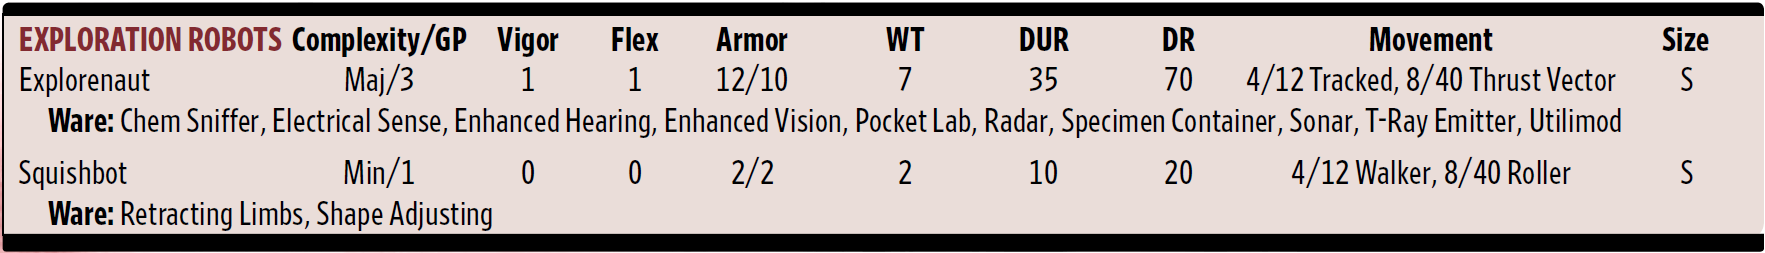
\includegraphics[width=\textwidth]{img/explorationRobots.png}
\end{figure}

\begin{itemize}
    \item \textbf{Chem Sniffer:} “This sensor detects molecules in the air and analyzes their chemical composition, using Know: Chemistry 60. It can determine the presence of explosives, firearms, and gases — including toxins and other fumes. Chemical Sniffers: In addition to detecting explosives and weapons, sniffers can be set to detect the carbon dioxide exhaled in transhuman breaths. This is useful for detecting intruding biomorphs in areas that are abandoned/off-limits.” \citep[pg. 318, 373]{ep2e_1.1_2019}

    \item \textbf{Electrical Sense:} “You can sense electric fields. Within 5 meters, you can tell if a device is on or off and can detect the precise location of electrical wiring and power supplies behind a wall or inside a device.” \citep[pg. 318]{ep2e_1.1_2019}

    \item \textbf{Enhanced Hearing:} “The morph’s ears can hear both higher and lower frequency sounds — the range of sounds they can hear is twice that of normal human ears (Senses and Sensors $\blacktriangleright$318). Your hearing is also more sensitive, allowing you to hear sounds as if you are 5 times closer. Apply a +10 to hearing-based Perceive Tests.” \citep[pg. 318]{ep2e_1.1_2019}

    \item \textbf{Enhanced Vision:} “The morph’s eyes have tetrachromatic vision capable of exceptional color differentiation. These eyes can also see the electromagnetic spectrum from terahertz wave frequencies to gamma rays, enabling them to see a total of several dozen colors, instead of the seven ordinary human eyes can perceive (Senses and Sensors $\blacktriangleright$318). In addition, these eyes have a variable focus equivalent to 5 power magnifiers or binoculars. You can also selectively filter what frequencies you perceive to avoid minor distractions on those wavelengths. This augmentation provides a +10 modifier to all Perceive Tests involving vision.”  \citep[pg. 318]{ep2e_1.1_2019}

    \item \textbf{Pocket Lab:} “This small handheld device contains numerous sensors for analyzing both organic and inorganic compounds in liquid, gaseous, and solid form. It performs material analysis using different methods of spectrometry, chromatography, and biochemical testing, comparing results to a built-in database. Using a pocket lab you could test soil fertility, identify clean water, detect hazardous emissions, discover traces of life, pinpoint contaminants, determine the presence of explosives or firearms, identify strange substances, and so on. It operates with Know: Chemistry 60.” \citep[pg. 340]{ep2e_1.1_2019}

    \item \textbf{Radar:} “This sensor system bounces radio or microwaves off targets and measures the reflected waves to judge size, composition, and motion (Senses and Sensors $\blacktriangleright$318).” \citep[pg. 318]{ep2e_1.1_2019}

    \item \textbf{Specimen Container:} “This capsule container is designed to hold samples of any sort (chemical, biological, etc.) in near stasis. It can be programmed to reproduce whatever conditions the user specifies, from cryogenic freezing to extreme heat, or even vacuum or high-pressure atmosphere. The containers are also encased in a superconductive wire mesh that acts as a faraday cage and blocks mesh and radio signals and similar electromagnetic radiation.” \citep[pg. 340]{ep2e_1.1_2019}

    \item \textbf{Sonar:} “You possess echolocation like a bat or dolphin. You bounce ultrasonic pulses off your surroundings and measure the echoes to build an image of the environment (Senses and Sensors $\blacktriangleright$318). This augmentation works in both air and water, out to a range of 20 (air) or 100 (water) meters.” \citep[pg. 318]{ep2e_1.1_2019}

    \item \textbf{T-Ray Emitter:} “Mounted under the skin of the user’s forehead, this implant generates low-powered beams of terahertz radiation (t-rays). Characters with enhanced vision can use reflected t-rays to see effectively see through walls and other materials (Senses and Sensors $\blacktriangleright$318). This implant allows the user to see using reflected t-rays for 20 meters in a normal atmosphere and for 100 meters in vacuum.” \citep[pg. 318]{ep2e_1.1_2019}

    \item \textbf{Utilimod:} “This mod duplicates the functions of a utilitool $\blacktriangleright$317. Retractable smart material tool “arms” are implanted — usually spaced around the wrist, but other locations are possible — that can change shape into almost any type of specialized tool desired in 1d6 minutes. These tools can take on numerous functions, including that of a fiber eye $\blacktriangleright$338 or an implanted knife $\blacktriangleright$204. Utilitool: In its basic form, a utilitool is the size and shape of a large fountain pen. Made from smart materials, it can transform into almost any tool in 1d6 minutes, from a wrench, knife, or powered screwdriver to a rotary grinder or pair of pliers.” \citep[pg. 325]{ep2e_1.1_2019}
\end{itemize}

“All bots are equipped with the following hardware, in addition to that listed with their specific description:”

\begin{itemize}
    \item \textbf{360° Vision:} “The morph’s eyes/visual sensors are situated for a 360-degree field of vision.” \citep[pg. 318]{ep2e_1.1_2019}

    \item \textbf{Access Jacks:} “Usually placed at the base of the skull, this external socket allows a direct neural interface with a cyberbrain or mesh inserts. A retractable fiberoptic cable enables you to plug into devices to access them directly, or to create a direct wired link to another person, allowing you to speak mind-to-mind and exchange data without fear of wireless sniffing. Access jacks are installed with all cyberbrains (and thus all pods and synthmorphs) by default.” \citep[pg. 318]{ep2e_1.1_2019}

    \item \textbf{Bot/Vehicle ALI:} “These AIs can pilot and control the bot/vehicle they are designed for without transhuman assistance. Autonomous Mode: Bot and vehicle shells are equipped with Bot/Vehicle ALIs $\blacktriangleright$326. In autonomous mode, the drone’s AI operates on its own, though it also follows commands issued verbally or via a communications link or entoptic control panel by an authorized entity. Issuing a one-sentence command is a mental quick action; commands can be issued to multiple drones at once. More complex commands may take longer, or can be prepared in advance with a Program Test. The AI may need to pass a COG Check to understand especially confusing or incomplete commands. Autonomous drones use their own Initiative, skills, and pools.” \citep[pg. 326, 346]{ep2e_1.1_2019}

    \item \textbf{Lidar:} “This sensor scans the area with laser light and measures the reflections to judge range, speed, and image the target (Senses and Sensors $\blacktriangleright$318). Lidar lasers are visible to enhanced vision, and are considered rude to continually emit in certain company.” \citep[pg. 318]{ep2e_1.1_2019}

    \item \textbf{Mesh Inserts:} “This network of implants is mandatory for people who want to use augmented reality and link wirelessly to the mesh. The various components include: Cranial Computer: This host serves as the hub for your personal area network and is home to your muse. It manages your augmented reality input and processes XP data, enabling you to share your sensorium with others in real-time. It is loaded with basic apps and provides all the functions you would expect from a mobile device: file storage, search engine, media player, mesh browser, address book, e-mail, messaging, and so forth. Medical/Diagnostic Sensors: This array monitors your health, including heart rate, respiration, blood pressure, temperature, neural activity, ware status, and more. In synthmorphs, this system monitors system reports and error logs, heat, stress faults, and similar hardware statuses. Radio Transceiver: This connects your headware with other mesh devices within range (5 km urban areas/50 km open areas). You can access any of these functions simply by thinking.” \citep[pg. 316]{ep2e_1.1_2019}

    \item \textbf{Puppet Sock:} “Puppet socks allow a morph to be remotely controlled, just like a drone (Remote Operations $\blacktriangleright$346). While active, the puppet has no control over their body and is simply along for the ride. Too long in this situation can lead to stress from helplessness (Stressful Situations $\blacktriangleright$229). Morphs with damage that reaches/ exceeds their Durability cannot be puppeted.” \citep[pg. 316]{ep2e_1.1_2019}
\end{itemize}